%
% This file is part of Calicut University Question Paper Collection.
%
% Copyright (c) 2012-2015 Mohammed Sadik P. K. <sadiq (at) sadiqpk (d0t) org>.
% License: GNU GPLv3 or later
%
% Calicut University Question Paper Collection is free software: you can
% redistribute it and/or modify
% it under the terms of the GNU General Public License as published by
% the Free Software Foundation, either version 3 of the License, or
% (at your option) any later version.
% 
% Calicut University Question Paper Collection is distributed in the hope
% that it will be useful,
% but WITHOUT ANY WARRANTY; without even the implied warranty of
% MERCHANTABILITY or FITNESS FOR A PARTICULAR PURPOSE.  See the
% GNU General Public License for more details.
% 
% You should have received a copy of the GNU General Public License
% along with Calicut University Question Paper Collection.
% If not, see <http://www.gnu.org/licenses/>.
% 
%

\def \subj{AI 09 403---LINEAR INTEGRATED CIRCUITS AND APPLICATIONS}

\mainhead{C 40960}{2}
\semfour{APRIL 2013}
\sub{\subj}
\maxtime

\partA

\iitem What is a planar process?
\item Define CMRR and slew rate.
\item What is the purpose of current mirror? explain.
\item How zero-crossing detector works?
\item Design a notch filter for notch frequency of 60 Hz.

\markA
\partB

\item Explain about differential amplifier.
\item Explain the frequency response of Op-amp.
\item Explain the operation of V to I converter.
\item Explain the operation of squarewave generator.
\item Write a note on the switched capacitor filter.
\item Explain the working of timing mark generator.

\markB
\partC

\item Describe the fabrication of an IC using monolithic technology with
  suitable figures.
\Or
\item Discuss the large signal operation of differential amplifier and
  operation of Ga As amplifier.

\newpage \again

\item Analyse the DC and AC characteristic of Op-amp in detail.
\Or
\item Explain the internal circuit of an Op-amp.

\item Explain the operation of Instrumentation amplifier, Integrator
 and logarithmic amplifier.
\Or
\item Discuss the working of precision rectifier, analog multiplier and
  V to I converter with grounded load.

\item Explain the design steps involved in design of Bandpass filter,
  universal active filter and Wien bridge oscillator.
\Or
\item Discuss briefly about Astable multivibrator, sawtooth generator
  and highpass filter.

\markC
\ene

\newpage

\mainhead{C 26896}{3}
\semfour{MAY 2012}
\sub{\subj}
\maxtime

\partA

\iitem What is surface mount technology?
\item Why current mirror is used as an active load?
\item For a peak detector, C = 0.01 $\mu$F, V$_i$ = 2V$_{pp}$ square wave at 1 kHz, draw the approximate
  output voltage.
\item Design a square wave oscillator for $f_\text{N}$ = 2 kHz. The Op-Amp supply is $\pm$15V.
\item Design a Notch filter for $f_{\text{N}}$ = 50 Hz.

\markA
\partB

\item Derive the expression of the current $\text{I}_{\text{R}}$ in Wilson current mirror.
\item For a non-inverting amplifier, $\text{R}_1$ = 100 $\Omega$, and R$_f$ = 10 k$\Omega$.
  Determine the maximum possible output offset voltage due to:
  \iitem Input offset voltage V$_{io}.$ \item Input bias current I$_{\text{B}}$.
    \ene
    The Op-Amp is LM307 ith V$_{io}$ = 10 mV and I$_\text{B}$ = 300 nA. What value of compensating
    resistor is needed to reduce the effect of input bias current I$_\text{B}$.
\item Design a circuit to implement the following: $\text{Y} = \dfrac{3\text{X}_1 +
  \text{X}_2}{\text{X}_3} + 4 \text{X}_4\text{X}_5 - \text{X}_6$, where Y is the output
  and $\text{X}_1, \text{X}_2 \dots \text{X}_6$ are the inputs to the circuit.
\item Design a Bandpass filter so that $f_o$ = 2 kHz, Q = 20 and A$_\text{o}$ = 10.

\newpage \again

\item Realize the following circuits with switched capacitors Fig. 1(a), 1(b):

\begin{tabular}{c c c c c}
& 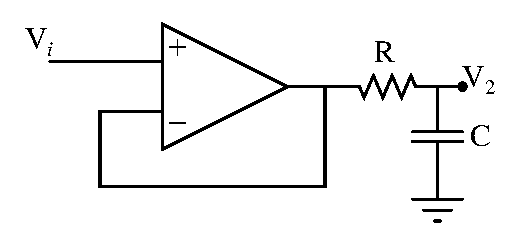
\includegraphics[scale=0.8]{src/s4/ai/09_403/fig001} & & 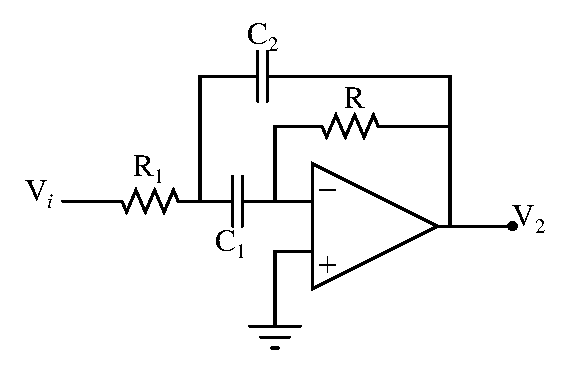
\includegraphics[scale=0.8]{src/s4/ai/09_403/fig002}\\
& \textbf{Fig. 1 (a)} &&  \textbf{Fig. 1 (b)}
\end{tabular}

\item For the input shown in Fig. 2 below, find the output of a differentiator if R$_f=2$k$\Omega$
  and C$_1=0.1\mu$F.

\begin{center}
 \begin{tabular}{c}
  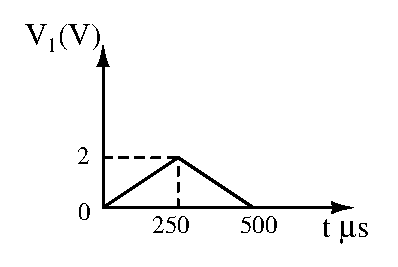
\includegraphics[scale=0.8]{src/s4/ai/09_403/fig003}\\
  \textbf{Fig. 2.}
 \end{tabular}
\end{center}

\markB
\partC

\item Describe the CMOS technology of fabricating an IC. \marko{10}
\Or 
\item Derive the expression for the output voltage and gain of a differential amplifier. \marko{10}

\item \iitem Explain the working of pole zero compensation network. \marko{4}
\item Explain the importance of the parameters CMRR, PSRR, Slew rate and Bias current.

 \marko{6}
\ene
\Or
\item Discuss in detail the internal circuit of 741.

\newpage

\item Explain the operation of the following circuits:
\iitem V to I converter
\item Timing mark generator
\item Peak detector
\ene
\Or
\item Describe the operation of Instrumentation amplifier, Logarithmic amplifier and Averaging amplifier.

\item \iitem Explain the operation of Astable multivibrator with suitable output waveform.  \marko{5}
\item Describe a fourth order Butterworth low pass filter having upper cut-off frequency 1kHz.

 \marko{5}
\ene
\Or
\item \iitem Derive the transfer function of a Band reject filter.
\item Design a monostable multivibrator with trigger pulse shaping which will drive an LED on for
      0.5 second each time it is pulsed. \ene

\markC
\ene

\newpage

\mainhead{C 15656}{2}
\semfour{JUNE 2011}
\sub{\subj}
\maxtime

\partA

\iitem What is the purpose of oxidation?
\item Why offset voltage is observed in an Op-amp?
\item Design an non-inverting amplifier with a gain of 3.
\item Design a Wien-bridge oscillation for a frequency of operation of 2 kHz.
\item What are the features of GaAs amplifier.

\markA
\partB

\item Explain the common mode operation of differential amplifier.
\item In an inverting amplifier $\text{R}_1 = 1$k$\Omega$. and $\text{R}_\text{f} = 100$k$\Omega$,
  the Op-Amp has the 
  following specifications: $\dfrac{\Delta\text{V}_{\text{OS}}}{\Delta \text{T}} =
  30\mu\text{V}/^{\circ}\text{C}$ max and 
  $\dfrac{\Delta \text{I}_{\text{OS}}}{\Delta \text{T}} = 0.3 $nA$/^{\circ}$C max. Assume
  that the amplifier is 
  nulled at 25$^\circ$C. Calculate the value of error voltage and output voltage
  $\text{V}_{\text{o}}$ at 35$^\circ$C
  if $\text{V}_{\text{i}}$ = 1 mV and $\text{V}_{\text{i}}$ = 5mV dc.

\item Find $\text{R}_1$ and $\text{R}_\text{f}$ of a lossy integrator so that the peak gain is
  40 dB and the gain is 6 dB down from its peak value when W = 10,000 rad/s.
\item Design an instrumentation amplifier to provide an output gain of 5. State the features
  of this amplifier.
\item Design a saw tooth generator to generate a frequency of 2 kHz.
\item Design a band filter with a $\text{f}_\text{L} = 500$ Hz, $\text{f}_\text{H} \simeq 200$ Hz.

\markB
\partC

\item Discuss the steps involved with fabrication of an IC using CMOS technology.
\Or
\item Discuss the operation of GaAs amplifier and MOS differential amplifier.

\newpage \again

\item Discuss the operation of internal circuit of an Op-Amp.
\Or
\item Explain briefly about the compensating networks used for offset voltages, bias currents and frequency 
  instability.

\item Write a note on the following I to V converter, Integrator and peak detector.
\Or
\item Explain the operation of summing amplifier, logarithmic amplifier and differentiator.

\item Explain the following Wien bridge oscillator, universal active filter and Notch filter.
\Or
\item Write briefly about switched capacitor filter, Astable multi-vibrator and low pass filter.

\markC
\ene
